\documentclass{beamer}
\usepackage{pgfpages}
\pgfpagesuselayout{4 on 1}[a4paper,border shrink=5mm,landscape]
\mode<presentation> {

%\usetheme{Montpellier}
\usetheme{PaloAlto}
\usecolortheme{whale}
\setbeamertemplate{footline}[page number]

}

\usepackage[utf8]{inputenc}
\usepackage{graphicx}
\usepackage{booktabs}
\usepackage{amsmath}
\usepackage{subfig}
\usepackage{caption}
\usepackage{xcolor, colortbl}
\usepackage{mathabx}
\usepackage{wrapfig}
\usepackage{tikz}
\usepackage{animate}
\usetikzlibrary{shapes.geometric, arrows}
\usepackage{listings}
\usepackage{verbatim}

\title[]{GTK+, une alternative à Qt}

\author{PÉRUTION-KIHLI Guillaume, RUSSO Judicaël}
\institute[Université de Montpellier]{Université de Montpellier \\ 
\medskip
}
\date{6 mars 2017}



\begin{document}

\maketitle

%----------------------------------------------------------------------------------
\begin{frame}{Sommaire}
  \tableofcontents
\end{frame}
%----------------------------------------------------------------------------------
\section{Introduction}
\begin{frame}{Historique}
  \begin{itemize}
  	\item GTK (GIMP ToolKit) est créé en 1997 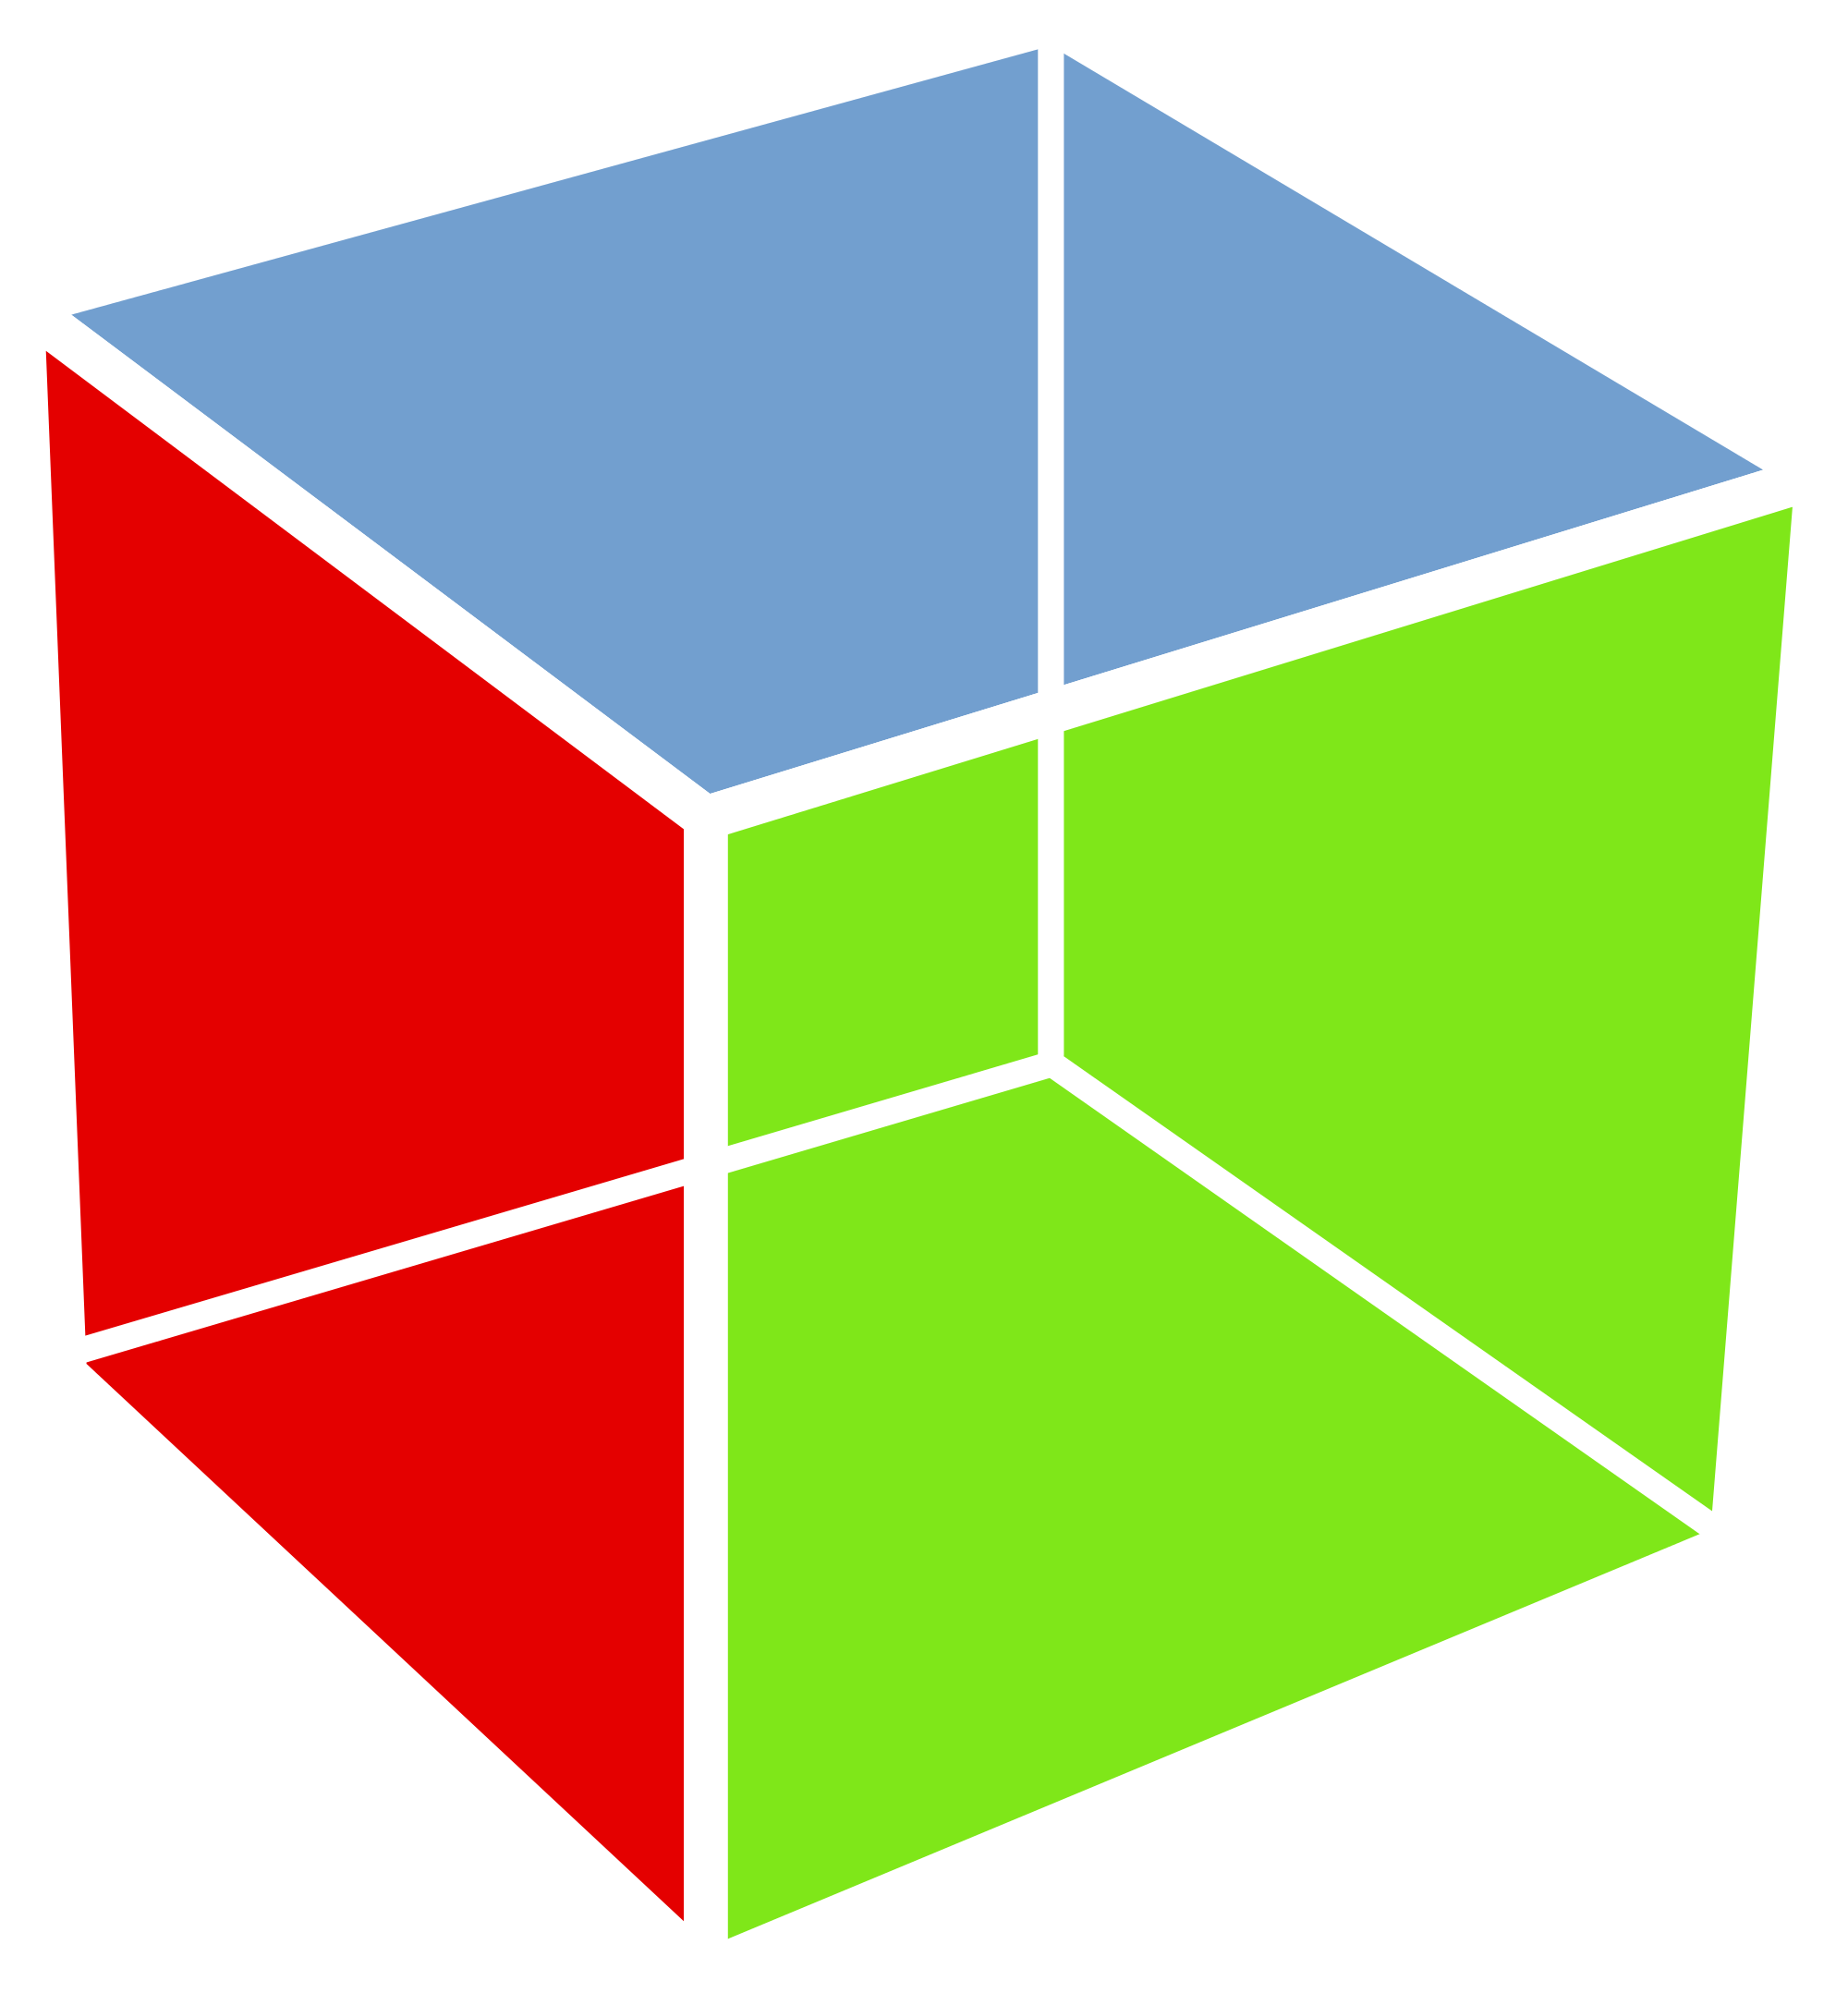
\includegraphics[scale=0.05]{Pictures/GTK.png} 
   \end{itemize}
\end{frame}
\begin{frame}{Historique}
  \begin{itemize}
  	\item GTK (GIMP ToolKit) est créé en 1997
    \item GIMP : Peter Mattis, Spencer Kimball, Berkeley 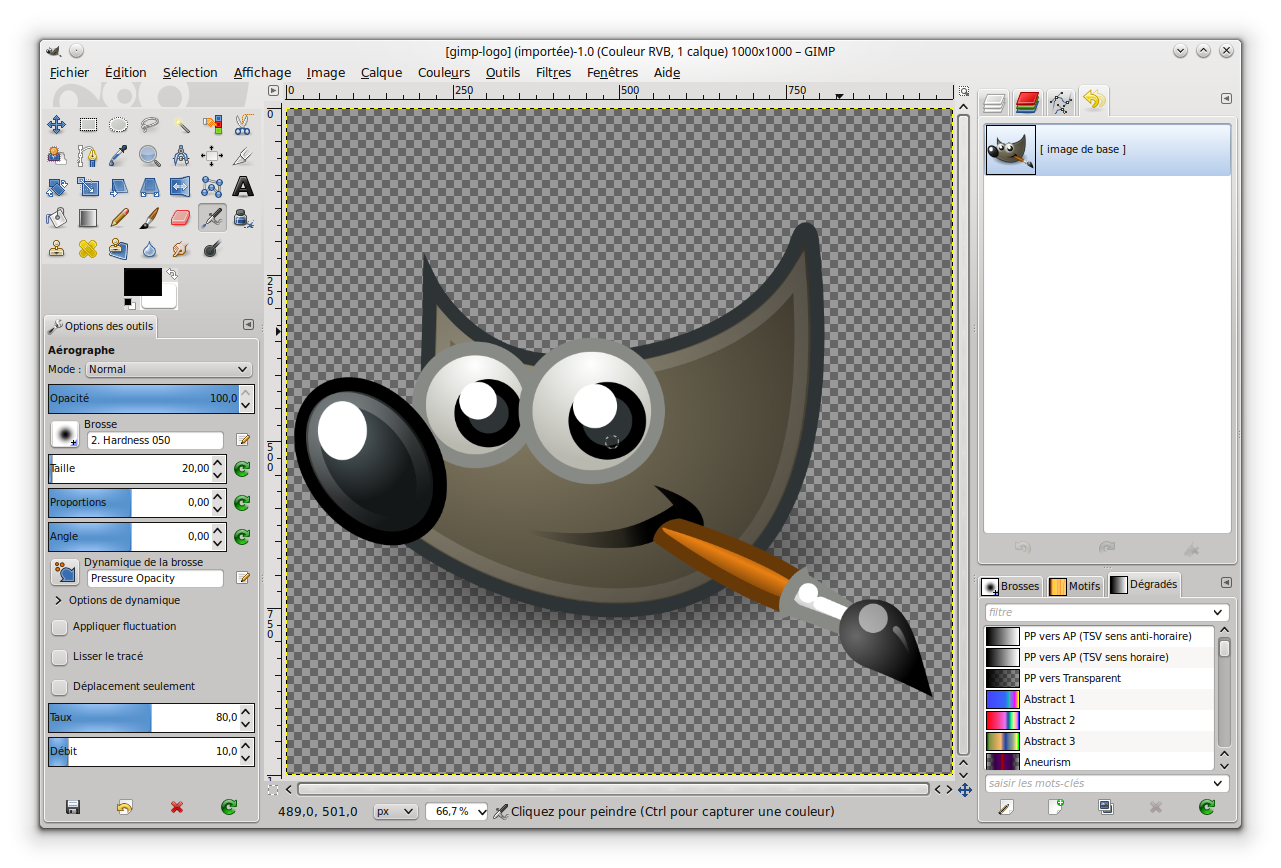
\includegraphics[scale=0.2]{Pictures/gimp.png} 
   \end{itemize}
\end{frame}
\begin{frame}{Historique}
  \begin{itemize}
  	\item GTK (GIMP ToolKit) est créé en 1997
    \item GIMP : Peter Mattis, Spencer Kimball, Berkeley 
    \item 1998 : GTK+ \pause
    \item 1999 : Création de GNOME \linebreak 
\includegraphics[scale=0.05]{Pictures/GNOME.png} 
   \end{itemize}
\end{frame}
\begin{frame}{Historique}
  \begin{itemize}
  	\item GTK (GIMP ToolKit) est créé en 1997
    \item GIMP : Peter Mattis, Spencer Kimball, Berkeley 
    \item 1998 : GTK+ 
    \item 1999 : Création de GNOME
    \item 2002 : GTK+ 2 / séparation avec GObject  \pause
    \item 2011 : GTK+ 3 
   \end{itemize}
\end{frame}

%---------------------------------------------------------------------------
\section{Présentation de GTK+}
\begin{frame}{GTK+, qu'est-ce que c'est ?}
	La bibliothèque GTK+ permet de réaliser des “GUI” (Graphical user interface), c’est-à-dire des interfaces graphiques pour des programmes. 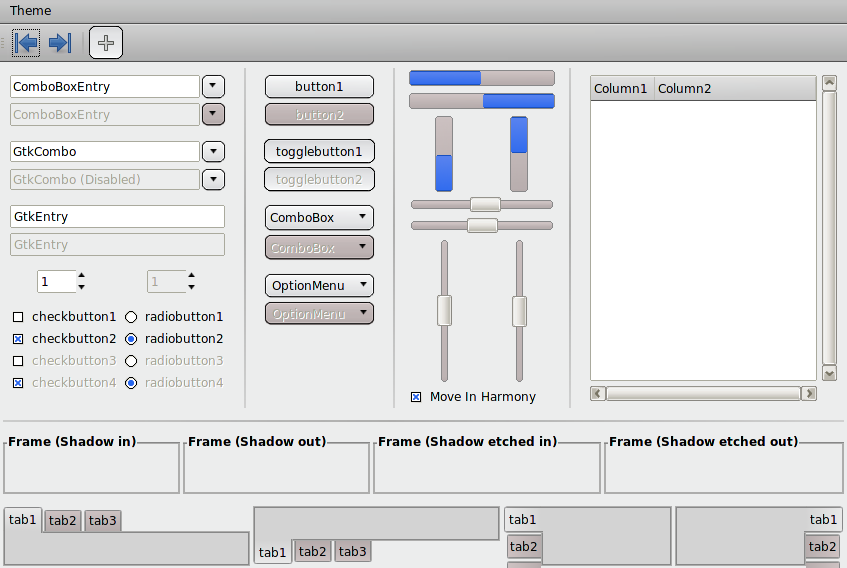
\includegraphics[scale=0.27]{Pictures/GTKExemple.png}
\end{frame}

%---------------------------------------------------------------------------

\begin{frame}{C et paradigme objet}
	\begin{itemize}
    \item GTK+ est programmé en C 
	\item GObject (GLib Object System), permet de programmer en orienté objet tout en utilisant n'importe quel compilateur C. \pause
    \item Mais cela n'est pas toujours optimal au niveau de l'écriture du code
	\end{itemize}
\end{frame}

%----------------------------------------------------------------------------
%---------------------------------------------------------------------------
\begin{frame}{Une bibliothèque portable}
	\begin{itemize}
	\item GTK+ est d'abord conçu pour fonctionner avec X11 et Wayland, environnements graphiques pour GNU/Linux 
\includegraphics[scale=0.075]{Pictures/X11.png} 
\includegraphics[scale=0.15]{Pictures/wayland.png} 
    \item Mais il fonctionne également sous d'autres environnements : Windows, MacOS \linebreak
 
\includegraphics[scale=0.15]{Pictures/os_x_windows_thumb800.jpg}

	\end{itemize}
\end{frame}

%---------------------------------------------------------------------------

\begin{frame}{Bindings}
	\begin{itemize}
      \item Principal binding : Gtkmm (GTK minus minus) qui permet le portage en C++  
      \item C\#  
      \item Java  
      \item etc ...
	\end{itemize}
\end{frame}

%---------------------------------------------------------------------------
%---------------------------------------------------------------------------
\begin{frame}{Quels logiciels utilisent GTK+ ?}
	\begin{itemize}
	\item Gnome  \linebreak  
\includegraphics[scale=0.01]{Pictures/GNOME.png}  \pause
    \item Unity, XFCE, MATE, LXDE  \linebreak 
\includegraphics[scale=0.15]{Pictures/Unity.png} 
\includegraphics[scale=0.05]{Pictures/Xfce_logo.png} 
\includegraphics[scale=0.15]{Pictures/mate.png} 
\includegraphics[scale=0.05]{Pictures/Lxde-logo2.png} \pause
    \item GIMP, firefox, pidgin...  \pause
    \item Mais certains logiciels et environnements ont abandonné GTK+ : Google Chrome, LXDE, Audacious, Openshot, etc
	\end{itemize}
\end{frame}

%---------------------------------------------------------------------------
%---------------------------------------------------------------------------
\begin{frame}{Outils de développement}
	\begin{itemize}
	\item Glade, permet de positionner des boutons ou fenêtres de manière graphique  \linebreak 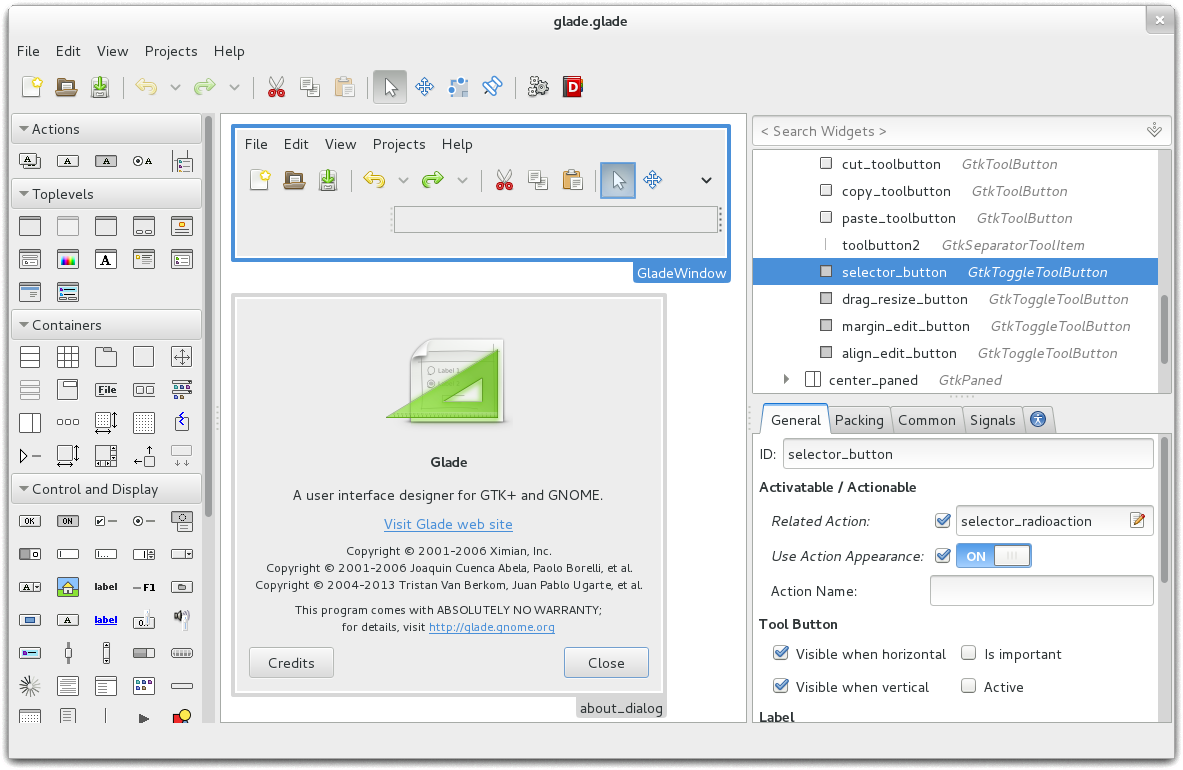
\includegraphics[scale=0.2]{Pictures/glade.png}
	\end{itemize}
\end{frame}
\begin{frame}{Outils de développement}
	\begin{itemize}
	\item Glade, permet de positionner des boutons ou fenêtres de manière graphique 
    \item GTK-Builder permet la même chose avec du XML  \pause
    \item GTK-Inspector permet le débogage dans une interface graphique (Observation des réactions et interactions des widgets, ...) \linebreak 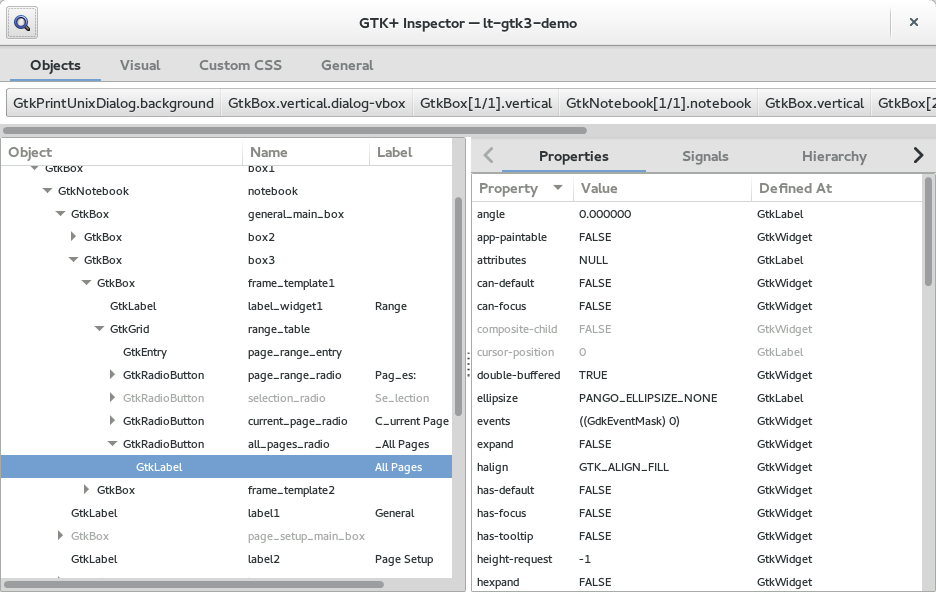
\includegraphics[scale=0.2]{Pictures/inspector.png}
	\end{itemize}
\end{frame}
\begin{frame}{Outils de développement}
	\begin{itemize}
	\item Glade, permet de positionner des boutons ou fenêtres de manière graphique  
    \item GTK-Builder permet la même chose avec du XML  
    \item GTK-Inspector permet le débogage dans une interface graphique (Observation des réactions et interactions des widgets, ...) 
    \item Il n'existe pas d'IDE officiel sous GTK+  
	\end{itemize}
\end{frame}

%---------------------------------------------------------------------------
\section{Une alternative crédible à Qt ?}
%---------------------------------------------------------------------------
\def \official{+++\cellcolor{green}}
\def \supported{+\cellcolor{green!50}}
\def \partially{-\cellcolor{blue}}
\def \unsupported{x\cellcolor{red}}

\begin{frame}{Bindings}
	\begin{table}[H]
\centering
	\begin{tabular}{| c | c | c | c |} \hline
    	Langage & GTK+ 2 & GTK+ 3 & Qt5 \\ \hline
        
        Ada & \unsupported & \unsupported & \official \\ \hline
        C\# & \partially & \unsupported & \supported \\ \hline
        C++ & \official & \supported  & \official \\ \hline
        D & \supported & \supported & \unsupported \\ \hline
        Fortran & \partially & \partially & \unsupported \\ \hline
        BASIC & \supported  & \supported & \supported \\ \hline
        Go & \partially & \partially & \supported \\ \hline
        Guile & \partially & \unsupported & \unsupported \\ \hline
        Haskell & \supported & \supported & \supported \\ \hline
        Java & \supported & \supported & \supported \\ \hline
        Javascript & \official & \official & \official \\ \hline
        Julia & \unsupported & \unsupported &\supported \\ \hline
        Lua & \unsupported & \supported & \supported \\  \hline
        
        
    \end{tabular}
\end{table}
    
\end{frame}
\begin{frame}{Bindings Suite}
	\begin{table}[H]
\centering
	\begin{tabular}{| c | c | c | c |} \hline
    	Langage & GTK+ 2 & GTK+ 3 & Qt5 \\ \hline
        
        OCaml & \partially & \unsupported & \unsupported \\ \hline
        Pascal & \supported & \supported & \unsupported \\ \hline
        Perl & \supported & \supported & \supported \\ \hline
        Python & \official & \official & \official \\ \hline
        PHP & \partially & \unsupported  & \unsupported \\ \hline
        QML & \unsupported & \unsupported & \official \\ \hline
        R & \partially & \unsupported & \unsupported \\ \hline
        Ring & \unsupported & \unsupported & \supported \\ \hline
        Ruby & \partially & \supported & \supported \\ \hline
        Rust & \unsupported & \supported & \supported \\ \hline
        Vala & \official & \official & \unsupported \\ \hline
        
        
    \end{tabular}
\end{table}
    
\end{frame}

%---------------------------------------------------------------------------
\begin{frame}{Portabilité}

	\begin{itemize}
	\item GTK+ est principalement conçu pour un environnement Linux. \pause
    \item Compatibilité seulement théorique \pause
    \item De nombreux processus de migration entamés récemment \pause
    \item Problèmes de rendus sous Windows et Mac OS X \pause
    \item Problèmes de support des appareils mobiles
	\end{itemize}

\end{frame}

\begin{frame}{Rétro-compatibilité}

	\begin{itemize}
	\item Incompatibilités entre GTK+ 3 et GTK+ 2 \pause
    \item Une transision de Qt4 à Qt5 beaucoup plus fluide
	\end{itemize}

\end{frame}

\begin{frame}{Consommation de ressources}
Configuration minimale de LXDE et LXQt.
	\begin{tabular}{|c|c|c|c|} \hline
    	Processeur & Ram & Disque Dur & Résultat \\ \hline
        Pentium II 266 MHz & 192Mo & 5400 tr/min & modérée-rapide \\ \hline
        VIA 400 MHz & 256Mo & 5400 tr/min & Modérée-rapide \\ \hline
        Pentium III 500MHz & 128Mo & 722 tr/min & potable \\ \hline
	\end{tabular}

\end{frame}

\begin{frame}{Outils de développement}

	\begin{itemize}
	\item QtCreator, un atout puissant 
\includegraphics[scale=0.05]{Pictures/Qtcreator.png} \pause
    \item Une séparation des couches métier avec Qt \pause
    \item QtDesigner vs Glade \pause
    \item QtTranslate 
	\end{itemize}

\end{frame}


\begin{frame}{Bibliographie}
  \begin{thebibliography}{10}
\setbeamertemplate{bibliography item}[online]
  \bibitem{A}
    \newblock Site officiel de GIMP
    \newblock https://www.gimp.org/
  \bibitem{A}
    \newblock Site officiel de GTK+
    \newblock https://www.gtk.org/
  \bibitem{A}
    \newblock Site officiel de Glade
    \newblock https://glade.gnome.org/
  \bibitem{A}
    \newblock Site officiel de LXDE
    \newblock http://lxde.org/
  \beamertemplatearticlebibitems\\
  \end{thebibliography}
\end{frame}
\end{document} 